\secnumberlesssection{ANEXOS}

\begin{itemize}
    \item Anexo 1:
        \\
        \vspace{3.5cm}
        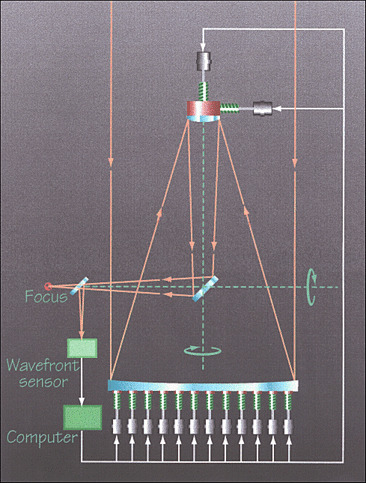
\includegraphics[width=6cm,height=9cm]{figures/actopt2.jpg} \\
        \vspace{3.5cm}


    \item Anexo 2:
        \\
        \vspace{3.5cm}
        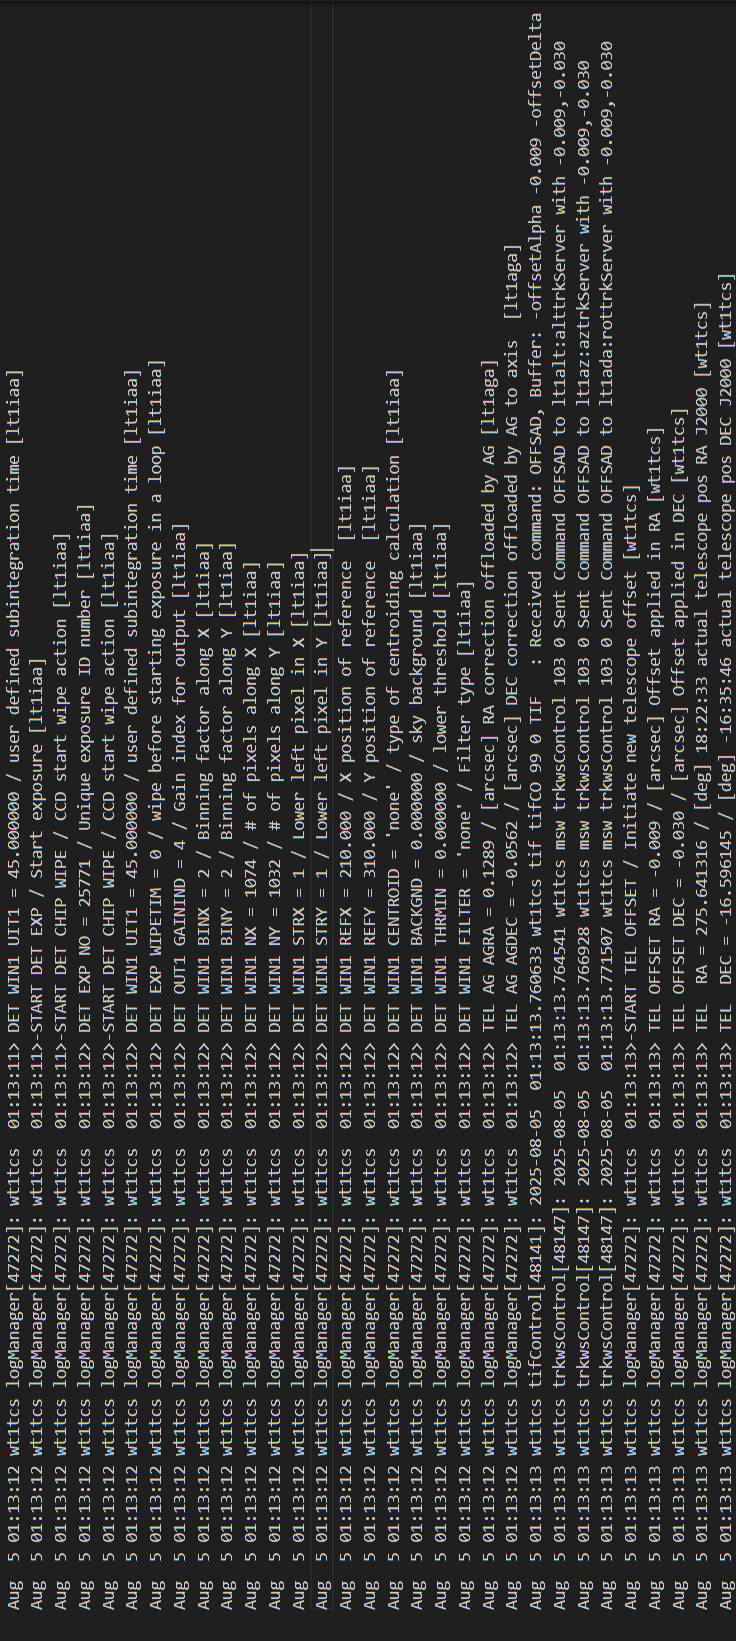
\includegraphics[width=12cm,height=18cm]{figures/log_vertical.png} \\
        \vspace{3.5cm}

    \item Anexo 3:
        \\
        \\
        \vspace{3.5cm}
        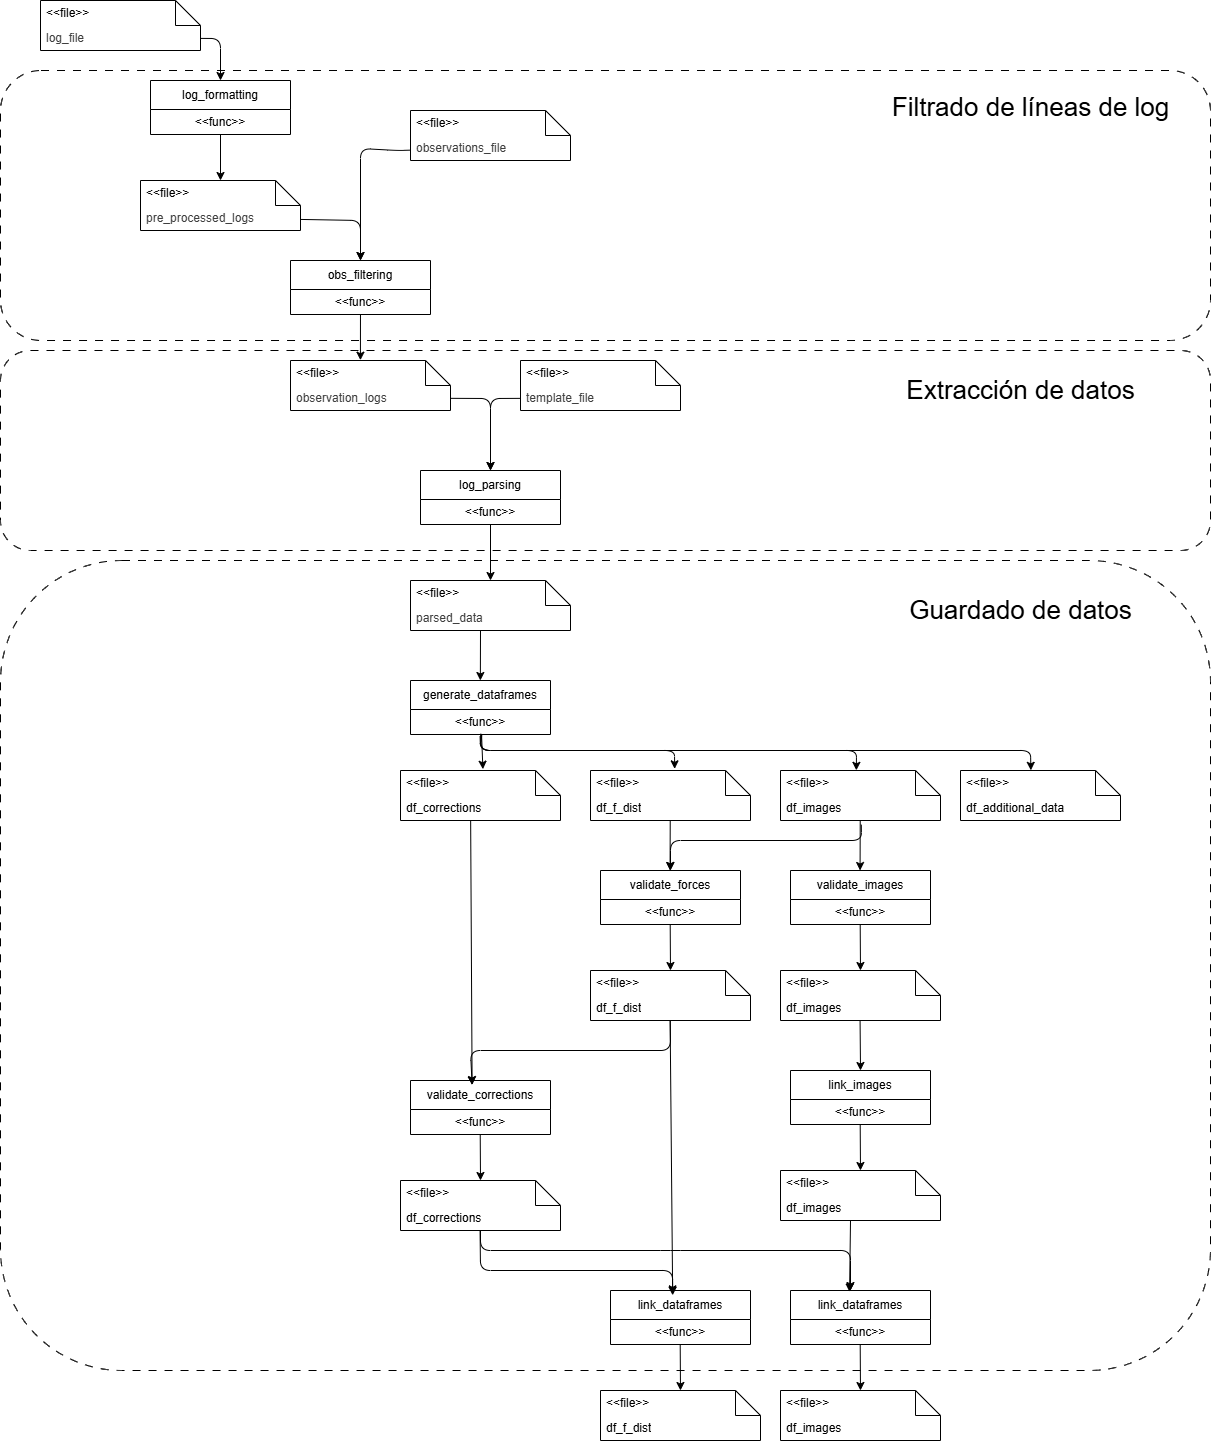
\includegraphics[width=12cm,height=16cm]{figures/flow_diagram.png} \\
        \vspace{3.5cm}

    \item Anexo 4:
        \\
        \\
        \vspace{3.5cm}
        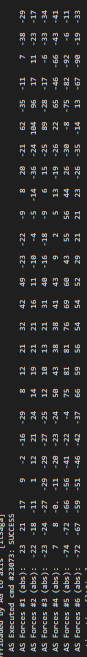
\includegraphics[width=2cm,height=16cm]{figures/log_f_dist.png} \\
        \vspace{3.5cm}
\end{itemize}


\begin{itemize}
    \item Diccionario 1: Frente de Onda

    El frente de onda es una superficie imaginaria que representa los puntos correspondientes de una onda que vibra al unisono. Cuando ondas idénticas con un origen en común viajan a través de un medio homogéneo, los senos y picos correspondientes a cada uno se mantienen en fase \cite{britannica2022front}. 

    \item Diccionario 2: Sensor de frente de onda

    Es un sensor diseñado para calcular las aberraciones de una imágen mientras se toma la misma. Generalmente las aberraciones son producidas por ladeos en los frentes de onda, presentes en imágenes que capturan objetos al otro lado de la atmósfera \cite{platt2001sh}

     \item Diccionario 3: Librería Template Text Parser

     Template Text Parser, o TTP, es una librería de Python que permite la extracción de datos de texto semi estructurado usando plantillas, manteniendo un rendimiento relativamente rápido. Iniclamente fue desarrollado para permitir el acceso procedural a datos producidos por las consolas de aparatos de red, sin embargo, actualmente puede ser usada para extraer cualquier texto semi estructurado que contenga patrones de repetición distintivos \cite{dmulyalin2021ttp}.
\end{itemize}